\chapter{Эволюция шланговой турбулентности магнитоактивной анизотропной плазмы 
}\label{ch:ch4}

\section{Деформация распределения частиц в зависимости от величины  внешнего магнитного поля}
\label{part_evol_distr_func}
В отсутствии внешнего магнитного поля и наклонных мод ранее наблюдалась значительная деформация функции распределения частиц на стадии насыщения экспоненциального роста во всей области скоростей порядка тепловых~\cite{Kuznetsov2023}. В данном процессе происходит быстрое увеличение поперечной к оси анизотропии скорости электронов, двигавшихся сначала преимущественно вдоль этой оси, так что его форма принимает вид, существенно отличный от бимаксвелловского~(рис. \ref{ris:FR_A10_3d_B0}). В дальнейшем форма функции распределения частиц, остающаяся сильно не бимаксвелловской, изменяется медленно, квазилинейно, т.е. исключительно за счет интегрального нелинейного влияния мод на однородную компоненту функции распределения в условиях формально линейной эволюции каждой моды согласно текущему значению инкремента (декремента) и частоты (в общем случае ненулевой), определяемыми этой медленно меняющейся функцией распределения частиц. Это было показано сравнением симуляций методом частиц в ячейках с расчетами, учитывающими исключительно квазилинейное взаимодействие. На временах, по меньшей мере пятикратно превышающих момент окончания экспоненциального роста, учет наклонных мод и нелинейных взаимодействий, с ними связанных, в отсутствие внешнего магнитного поля не оказывает существенного влияния на эволюцию распределения частиц по скоростям за исключением, возможно, кратковременного переходного промежутка примерно от $\omega_pt=80$ до $\omega_pt=100$ при насыщении неустойчивости. 


\begin{figure}[h!]
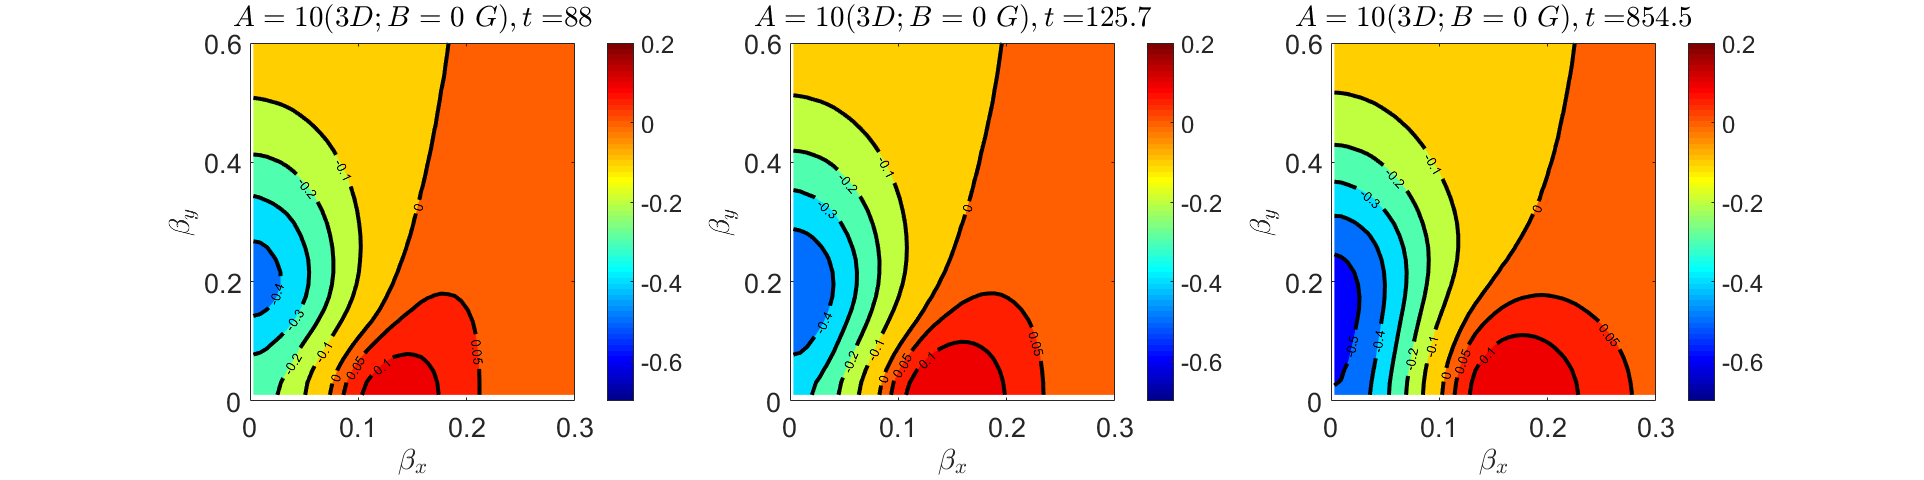
\includegraphics[width=1\linewidth]{part4/FR_B0_A10_3d.png}
\captionstyle{normal}
\caption{Вычисленные для моментов времени (a)~$\wpl t = 88$, (b)~$\wpl t = 125.7$, (c)~$\wpl t = 854.5$ линии уровня $-0.5$, $-0.4$, $-0.3$, $-0.2$, $-0.1$, $0$, $0.05$ и $0.1$ нормированной на максимум начального распределения поправки к однородной компоненте функции распределения (\ref{bimax}), которая в начальный момент времени являлась бимаксвелловской с параметром анизотропии $A_0=10$. Внешнее магнитное поле отсутствует: $b_{ext}=0$.}
\label{ris:FR_A10_3d_B0}
\end{figure}


В присутствии внешнего магнитного поля, по-прежнему, при насыщении неустойчивости происходит сравнительно быстрое увеличение поперечной к оси анизотропии скорости электронов, двигавшихся сначала преимущественно вдоль этой оси. С увеличением внешнего магнитного поля количество таких электронов уменьшается,  продольная скорость области их наибольшего прироста в момент насыщения неустойчивости увеличивается от нуля до $\beta_\|\sim3\beta_{\perp0}$, а поперечная остается примерно неизменной $\beta_\perp\lesssim2\beta_{\perp0}$ (рис. ~\ref{ris:FR_A10_3d_B78}). В ходе дальнейшего нелинейного развития турбулентности в отсутствие внешнего магнитного поля форма ФР частиц по скоростям меняется слабо, преимущественно за счет нагрева в поперечном к оси анизотропии направлении электронов с малой продольной скоростью, что расширяет область значительного оттока частиц в диапазон малых скоростей $\left(\beta_\perp<\beta_{\perp0},\beta_\|<\beta_{\|0}\right)$ (рис. \ref{ris:FR_A10_3d_B44}). Посредством сравнения трехмерных и двумерных аксиально симметричных расчетов кодом EPOCH с квазилинейным моделированием, в котором исключено прямое нелинейное взаимодействие между модами и оставлено лишь квазилинейное взаимодействие, было выявлено, что хотя к моменту насыщения неустойчивости указанные распределения частиц аналогичны, на более поздних временах они качественно отличаются в диапазоне малых скоростей  (ср. рис. \ref{ris:FR_A10_3d_B44_QL} и рис. \ref{ris:FR_A10_3d_B44}). Эта разница определяется существенно отличной динамикой спектра в обсуждаемых симуляциях (см. раздел \ref{part_spectr_b4}). Из этих различий следует, что квазилинейное приближение недостаточно для описания эволюции турбулентности  уже при довольно слабом внешнем магнитном поле, например, $b_{ext}=0.4$ при $A_0=10$. 

\begin{figure}[h!]
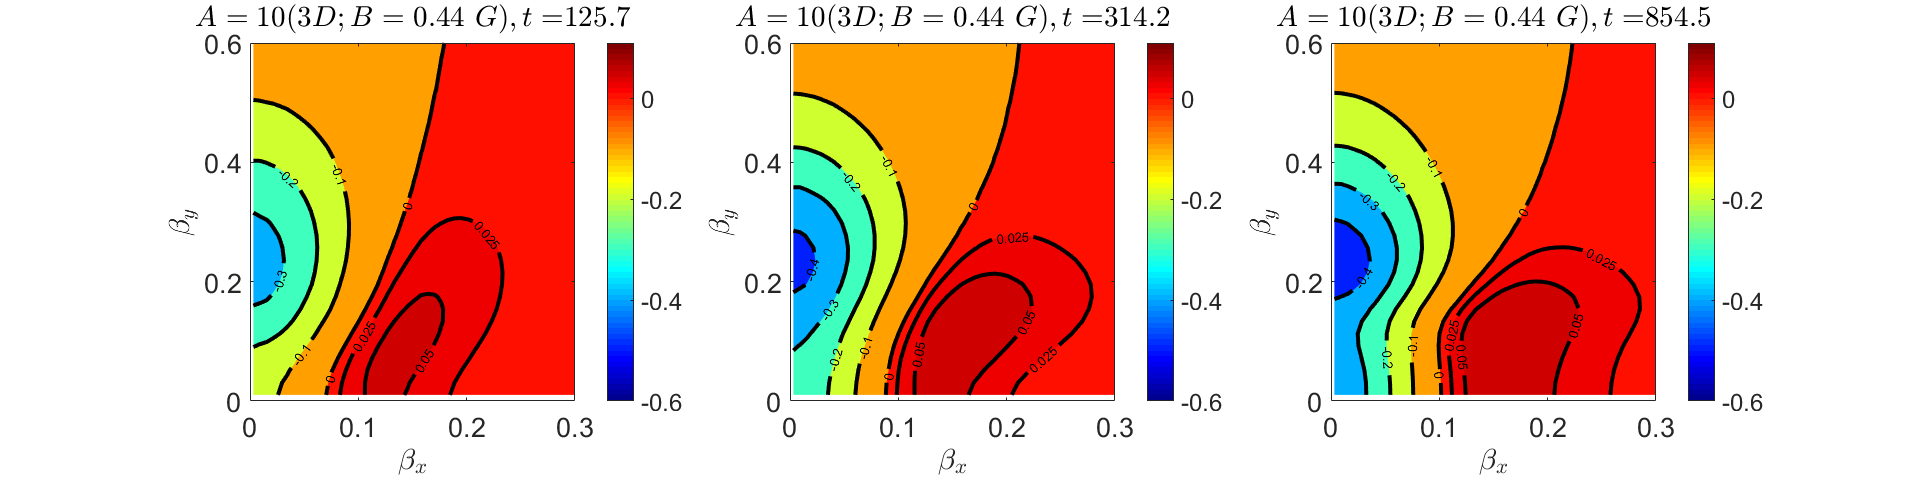
\includegraphics[width=1\linewidth]{part4/FR_B044_A10_3d.png}
\captionstyle{normal}
\caption{Вычисленные для моментов времени (a)~$\wpl t = 125.7$, (b)~$\wpl t = 314.2$, (c)~$\wpl t = 854.5$ линии уровня $-0.4$, $-0.3$, $-0.2$, $-0.1$, $0$, $0.025$ и $0.05$ нормированной на максимум начального распределения поправки к однородной компоненте функции распределения (\ref{bimax}), которая в начальный момент времени являлась бимаксвелловской с параметром анизотропии $A_0=10$. Внешнее магнитное поле $b_{ext}=0.4$.}
\label{ris:FR_A10_3d_B44}
\end{figure}

\begin{figure}[h!]

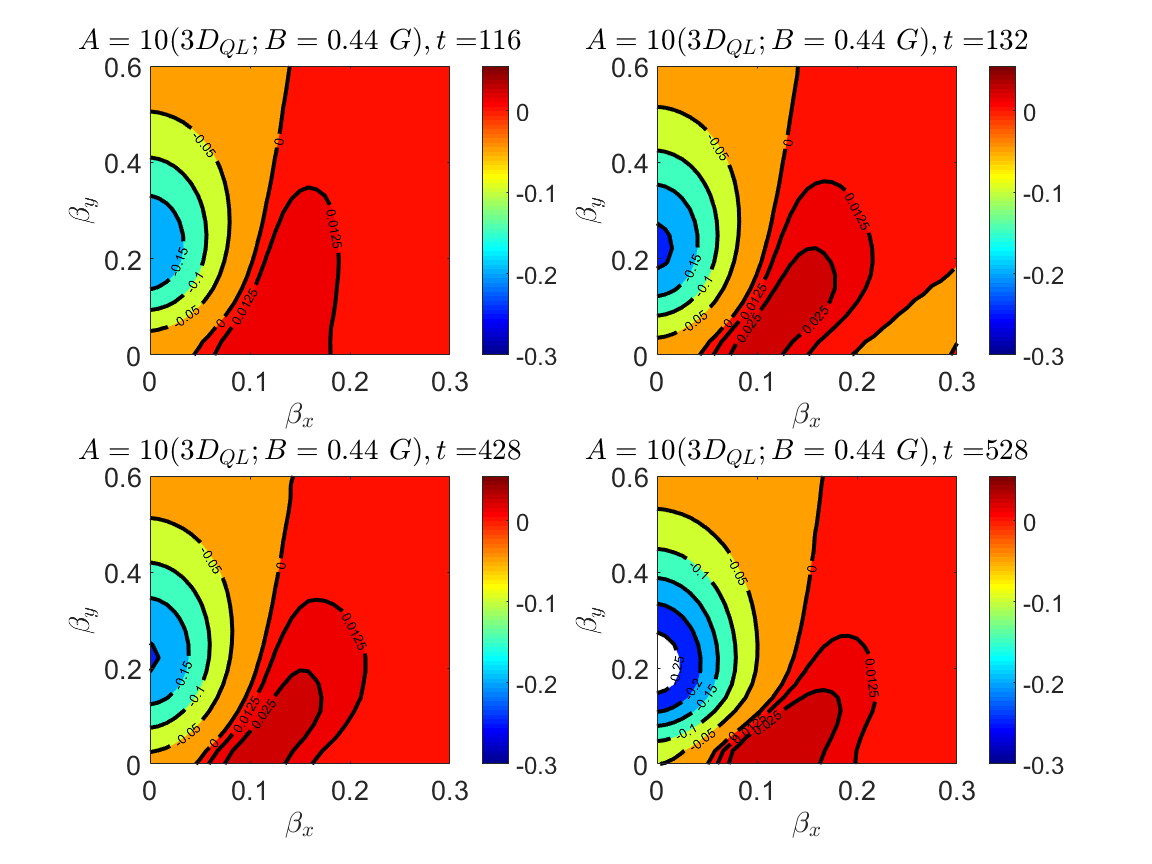
\includegraphics[width=1\linewidth]{part4/FR_QL_B4_A10.png}
\captionstyle{normal}
\caption{Вычисленные в квазилинейном аксиально симметричном приближении~\cite{Kuznetsov2023} для моментов времени (a)~$\wpl t = 84$, (b)~$\wpl t = 92$, (c)~$\wpl t = 100$, (d)~$\wpl t = 420$ линии уровня $-0.5$, $-0.4$, $-0.3$, $-0.2$, $-0.1$, $0$, $0.05$ и $0.1$ нормированной на максимум начального распределения поправки к однородной компоненте функции распределения (\ref{bimax}), которая в начальный момент времени являлась бимаксвелловской с параметром анизотропии $A_0=10$. Внешнее магнитное поле $b_{ext}=0.4$.}
\label{ris:FR_A10_3d_B44_QL}
\end{figure}

Нелинейное долговременное изменение ФР становится всё более заметным с увеличением магнитного поля: при $b_{ext}=0.71$ деформация ФР происходит преимущественно значительно позднее насыщения линейной апериодической неустойчивости. Продольная скорость расширяющейся области  наибольшего прироста снижается с $\beta_\|\sim3\beta_{\perp0}$ до $\beta_\|\sim2\beta_{\perp0}$, а поперечная почти не меняется.  Область значительного оттока частиц, абсолютный максимум которого достигается при $\beta_\|\sim3\beta_{\perp0}$,  также существенно расширяется на нелинейной стадии, причем появляется локальный максимум в области малых скоростей $\left(\beta_\perp<\beta_{\perp0},\beta_\|<\beta_{\|0}\right)$.
\begin{figure}[h!]

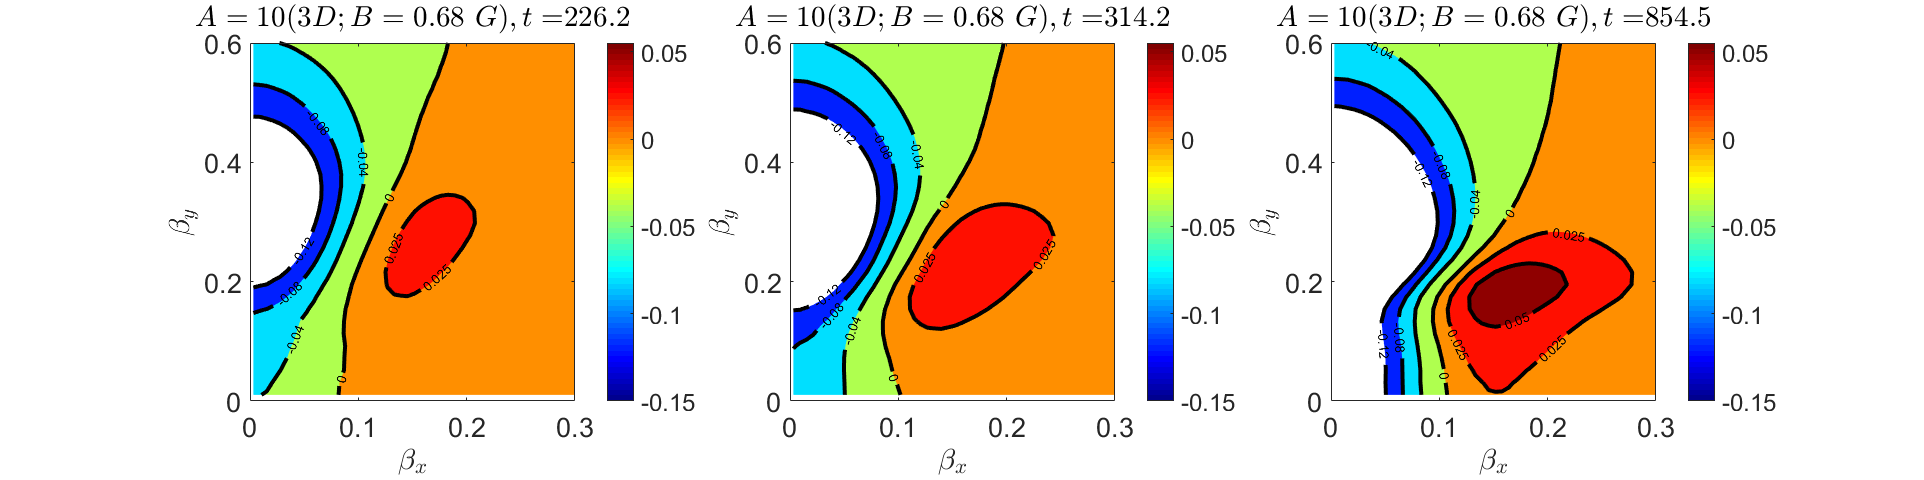
\includegraphics[width=1\linewidth]{part4/FR_B065_A10_3d.png}
\captionstyle{normal}
\caption{Вычисленные для моментов времени (a)~$\wpl t = 226.2$, (b)~$\wpl t = 314.2$, (c)~$\wpl t = 854.5$ линии уровня $-0.4$, $-0.3$, $-0.2$, $-0.1$, $0$, $0.025$ и $0.05$ нормированной на максимум начального распределения поправки к однородной компоненте функции распределения (\ref{bimax}), которая в начальный момент времени являлась бимаксвелловской с параметром анизотропии $A_0=10$. Внешнее магнитное поле $b_{ext}=0.59$.}
\label{ris:FR_A10_3d_B65}
\end{figure}


\begin{figure}[h!]
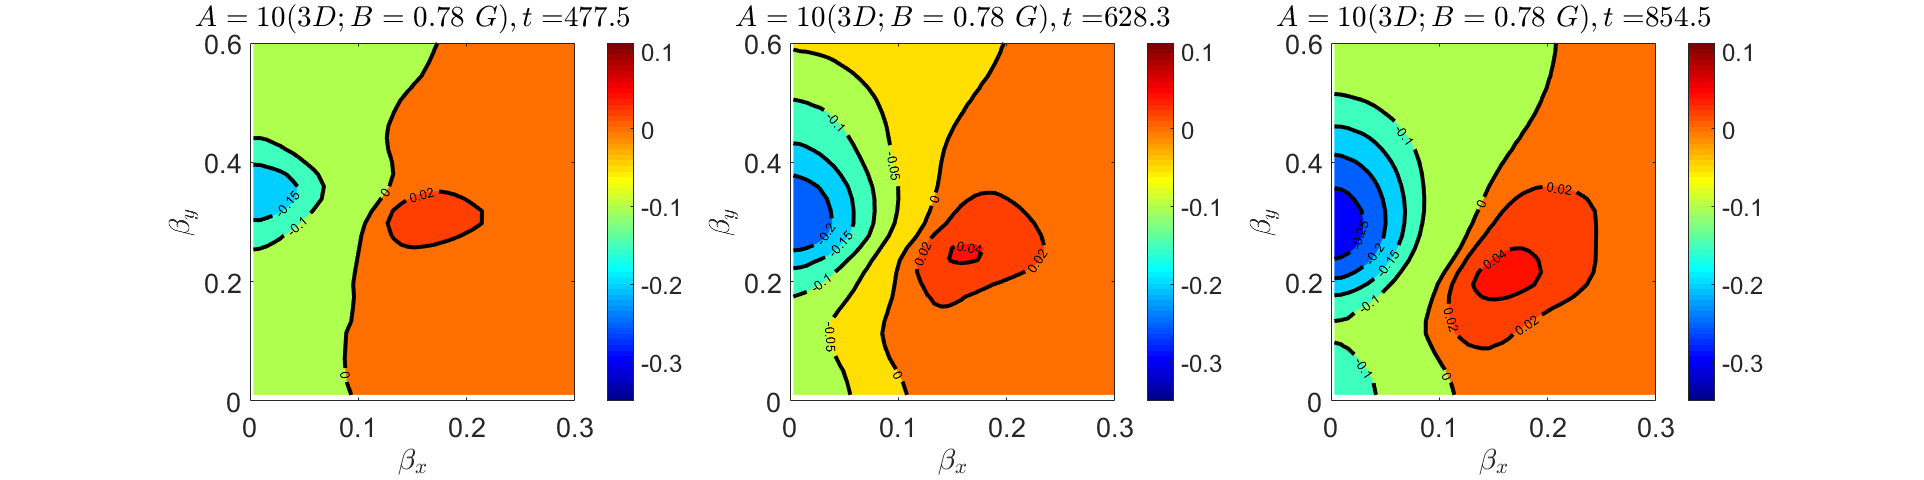
\includegraphics[width=1\linewidth]{part4/FR_B078_A10_3d.png}
\captionstyle{normal}
\caption{Вычисленные для моментов времени (a)~$\wpl t = 477.5$, (b)~$\wpl t = 628.3$, (c)~$\wpl t = 854.5$ линии уровня $-0.25$, $-0.2$, $-0.15$, $-0.1$, $-0.05$, $0$, $0.02$ и $0.04$ нормированной на максимум начального распределения поправки к однородной компоненте функции распределения (\ref{bimax}), которая в начальный момент времени являлась бимаксвелловской с параметром анизотропии $A_0=10$. Внешнее магнитное поле $b_{ext}=0.71$.}
\label{ris:FR_A10_3d_B78}
\end{figure}

Функции распределения частиц по скоростям в двумерных расчетах 2D3V с магнитным полем, лежащим в плоскости моделирования, демонстрируют качественно схожую динамику. Наиболее значительные отличия наблюдаются в отсутствие внешнего магнитного поля:  ФР в 2D3V-расчете теряет аксиальную симметрию, изотропизуясь лишь в плоскости, ортогональной к перпендикулярным волновым векторам. В присутствии внешнего магнитного поля распределение частиц испытывает ларморовское вращение и посредством этого приобретает возможность изотропизоваться в обоих перпендикулярных к оси анизотропии направлениях, стремясь, что особенно ярко выражено в сильном внешнем магнитном поле, к аксиально симметричному виду, аналогичному распределению частиц в трехмерных симуляциях. 


\section{Эволюция интегральных характеристик турбулентности при различных значениях внешнего магнитного поля}
\label{part_evol_aver}


Параметр анизотропии $A$, будучи интегральным отражением формы распределения частиц, в отсутствие внешнего магнитного поля испытывает наиболее значительное снижение к моменту насыщения неустойчивости, а в сильном магнитном поле, равном, например, $b_{ext}=0.71$, ситуация противоположная и изотропизация распределения происходит преимущественно в ходе нелинейной эволюции (рис. \ref{ris:average_A10}b). Так, в первом случае к насыщению неустойчивости в $\tau_s=88$ анизотропия резко, примерно в 5 раз, уменьшается до $\approx2$, далее её снижение плавно замедляется и на временах $2\tau_s=176$ она составляет $A\approx1.1$. Во втором случае к моменту насыщения неустойчивости $\tau_s=390$ анизотропия снижается всего до $\approx7.2$, а на временах $2\tau_s=780$ составляет уже $A\approx3.83$.

Тем интереснее, что величина среднеквадратичного магнитного поля к концу симуляции в этих противоположных случаях различалась всего на $5 \%$ (рис. \ref{ris:average_A10}a,d). В отсутствие внешнего поля эта величина сравнительно быстро выросла, достигла насыщения и начала быстро затухать. В сильном же внешнем поле апериодическая неустойчивость достигла своего насыщения в $4$ раза позднее и при в $3.5$ раза меньшем турбулентном магнитном поле, однако после этого  среднеквадратичное магнитное поле до конца симуляции находилось на примерно одном и том же уровне, что предопределило близость обсуждаемых величин к концу обеих симуляций. Полученное совпадение не выглядит случайным, так как среднеквадратичное магнитное поле в двух других расчетах с промежуточными значениями магнитного поля $b_{ext}=0.4$ и $b_{ext}=0.59$ к концу симуляции пришло к сравнимым значениям, отличающимся всего на $10 \%$ и $20 \%$ соответственно. Идентичный результат наблюдается и для аналогичных симуляций при начальной анизотропии $A_0=1$. Это позволяет предполагать, что внешнее магнитное поле, неизбежно присутствующее в корональных петлях, хотя и существенно меняет динамику турбулентного магнитного поля непосредственно после насыщения неустойчивости, слабо влияет на среднеквадратичную величину последнего на глубоко нелинейных временах, на которых масштабы турбулентности во всех направлениях сопоставимы. 
\begin{figure}[h]
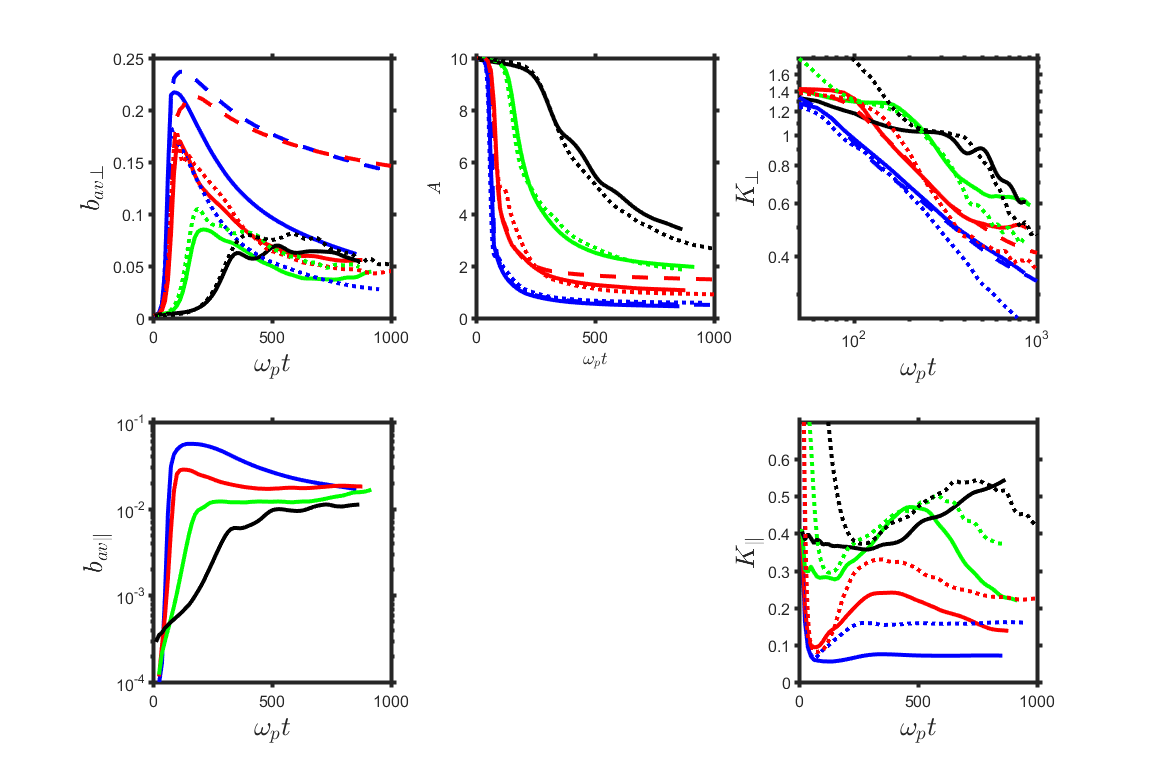
\includegraphics[width=1\linewidth]{part4/average_A10.png}
\captionstyle{normal}
\caption{Эволюция (a) поперечной и (d) продольной компонент среднеквадратичного магнитного поля $b_{av}$, (b) параметра анизотропии $A$, характерных (c) поперечной $\langle K_\perp\rangle$ и (f) продольной $\langle K_\|\rangle$ компонент волнового числа при значениях внешнего магнитного поля $b_{ext}=0$ (синий цвет), $b_{ext}=0.4$ (красный цвет), $b_{ext}=0.59$ (зеленый цвет) и $b_{ext}=0.71$ (черный цвет) в трехмерных (сплошная линия), двумерных с наклонными модами (пунктир) и двумерных аксиально симметричных (штрихи) симуляциях. Начальная анизотропия равна $A_0=10$.}
\label{ris:average_A10}
\end{figure}

Во всех трехмерных симуляциях преобладает поперечная к оси анизотропии компонента магнитного поля, кратно, но не на порядки превосходя продольную компоненту. На протяжении нелинейной эволюции турбулентности их отношение уменьшается. Так, в отсутствие внешнего магнитного поля при насыщении неустойчивости их отношение примерно равно $b_\perp/b_\|\approx4$, на момент окончания расчета~--- $b_\perp/b_\|\approx3$, а в сильном внешнем магнитном поле $b_{ext}=0.71$ при насыщении неустойчивости их отношение примерно равно $b_\perp/b_\|\approx10$,  на момент окончания расчета~--- $b_\perp/b_\|\approx5$. 

Значения характерных перпендикулярного $\langle K_\perp\rangle$ и продольного $\langle K_\|\rangle$ волновых чисел к моменту насыщения неустойчивости соответствуют волновому вектору наиболее неустойчивой моды, а значит, определяются линейной теорией. Здесь усреднение понимается в следующем смысле:
\begin{equation}
\label{eq:angles}
\langle...\rangle=\frac{\iiint\limits_0^\infty...b_K^2 d^3K}{\iiint\limits_0^\infty b_K^2 d^3K} ,
\end{equation}
Первое увеличивается c ростом внешнего магнитного поля, пока наиболее неустойчивыми модами остаются поперечные моды. При дальнейшем увеличении внешнего магнитного поля определяющими всю динамику турбулентности становятся наклонные моды, а характерное перпендикулярное волновое число снижается. Характерное продольное волновое число $\langle K_\|\rangle$в момент насыщения неустойчивости с ростом внешнего магнитного поля увеличивается.

В ходе последующей нелинейной эволюции поперечный масштаб турбулентности практически монотонно возрастает (рис. \ref{ris:average_A10}с и рис. \ref{ris:average_A10}f). Продольный масштаб сначала убывает вследствие нелинейного возбуждения разнообразных наклонных мод, устойчивых согласно линейной теории, а затем тоже возрастает. К концу симуляции во всех случаях продольный и поперечный масштабы оказывались сопоставимы, так что становится невозможно говорить о филаментационной структуре токов. В целом, результаты согласуются с~\cite{Hellinger2014,Camporeale2008}, отмечавшими увеличение масштаба турбулентности и уменьшение угла между внешним магнитным полем и характерным волновым вектором. Несмотря на хорошее количественное совпадение для всех четырех значений внешнего магнитного поля результатов эволюции параметра анизотропии (точность до 15\%) и среднеквадратичного магнитного поля (без случая $b_{ext}=0$ точность до 20 \%) у двумерных и трехмерных расчетов, сравнение в этих расчетах продольного и поперечного характерных масштабов турбулентности показывает, что на нелинейной стадии они значительно расходятся и могут кратно отличаться.  Это существенно затрудняет изучение долговременной спектральной эволюции трехмерной турбулентности на основе анализа двумерных симуляций, как это, по-видимому, делается в указанных выше работах. Анализ спектральной динамики турбулентности, генерируемой шланговой модой, ниже основан на трехмерных симуляциях и посвящен преимущественно спектральной динамике поперечной компоненты магнитного поля, усредненной по аксильному углу. Усреднение приводит к сглаживанию шумов и осцилляций, наблюдаемых на стадии затухания мод, что позволяет оценить показатель степенного спадания их амплитуды.

\section{Влияние внешнего магнитного поля на спектральную эволюцию шланговой турбулентности и нелинейные эффекты четырехволнового и трехволнового взаимодействия мод}
\subsection{Динамика спектра вейбелевской турбулентности и нелинейное взаимодействие мод в отсутствие внешнего магнитного поля}
\label{part_spectr_bo}


В отсутствие наклонных мод и внешнего магнитного поля общий сценарий эволюции спектра вейбелевской турбулентности, который по существу можно назвать квазилинейным, был подробно описан в работе~\cite{Kuznetsov2023} в аксиально симметричной двумерной геометрии (все моды лежат в плоскости, ортогональной к оси анизотропии). При бимаксвелловском начальном распределении частиц неустойчивой оказывается исключительно ТМ-мода, магнитное поле которой ортогонально к плоскости опредлеляемой осью анизотропии и волновым вектором. После насыщения неустойчивости спектр магнитного поля, управляемый преимущественно квазилинейным взаимодействием, смещается в длинноволновую область так, что характерное волновое число уменьшается степенным образом, а степень наклона длинноволнового и коротковолнового хвостов остается при.
мерно постоянной, что говорит об автомодельности динамики спектра. Единственным наблюдаемым нелинейным эффектом является развитие ТМ-гармоник, нечетным образом кратных к оптимальной, преимущественно утроенной гармоники, генерируемой четырехволновым взаимодействием~\cite{Garasev2021,Kuznetsov2023}. Таким образом, были выделены 4 стадии эволюции ТМ-мод: экспоненциальный рост согласно линейному дисперсионному уравнению, степенной рост мод, волновое число которых меньше характерного $\langle K_\perp\rangle$, осцилляционное затухание мод, волновое число которых больше характерного $\langle K_\perp\rangle$, и сверхбыстрый нелинейный рост вследствие четырехволнового взаимодействия~(рис. \ref{ris:all_modes}a).  Показатель степенного роста оценивался примерно от $1$ до $2$, а показатель затухания, которое после усреднения по аксиальному углу оказывалось степенным, лежал в небольшом диапазоне значений от $-1.3$ до $-1$ для широкого диапазона значений начальных анизотропий. 

\begin{figure}[h]
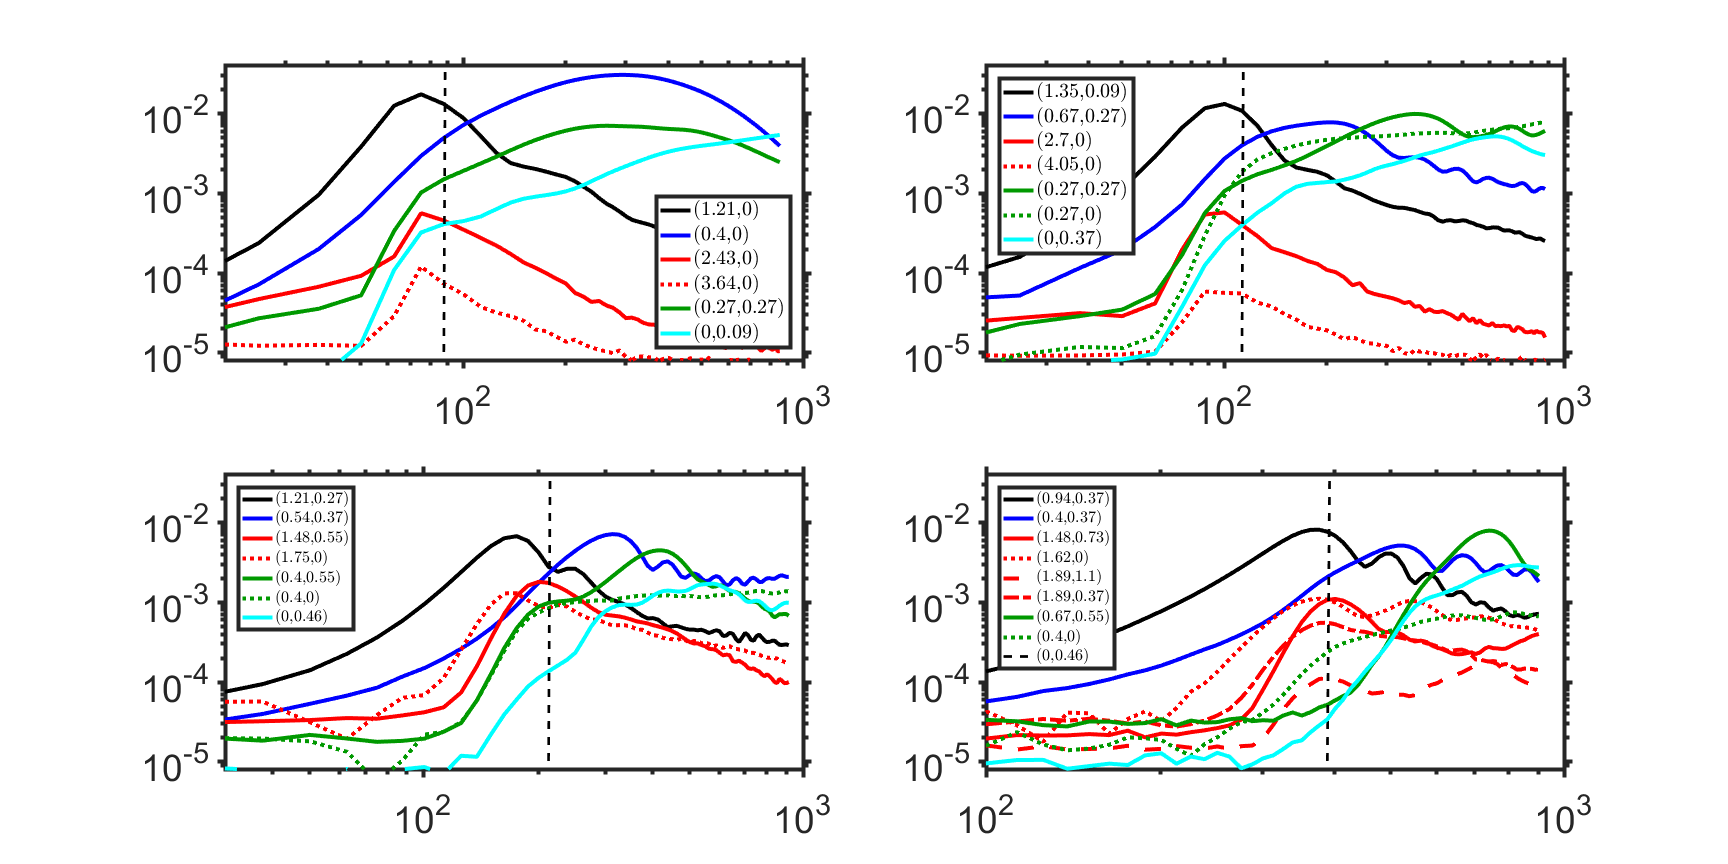
\includegraphics[width=1\linewidth]{part4/garmoniki_final.png}
\captionstyle{normal}
\caption{Эволюция типичных усредненных по аксиальному углу мод: примерно оптимальной моды $\overrightarrow{K}_{opt}$ (черный цвет); линейно неустойчивой моды, испытывающей степенное нарастание (синий цвет);  линейно устойчивых, затухающих непосредственно после сверхбыстрой генерации мод (красный цвет); линейно устойчивых, примерно степенным образом нарастающих после окончания сверхбыстрой генерации мод (зеленый цвет), наиболее энергонесущей моды с $K_\perp=0$ (бирюзовый цвет) при внешнем магнитном поле (a) $b_{ext}=0$, (b) $b_{ext}=0.4$. (c) $b_{ext}=0.59$, (d) $b_{ext}=0.71$. Вертикальный пунктир соответствует первому локальному максимуму среднеквадратичного магнитного поля в каждом случае. Начальная анизотропия $A_0=10$.}
\label{ris:all_modes}
\end{figure}

Другим нелинейным эффектом, который наблюдается в аксиально симметричной двумерной (как в работе \cite{Kuznetsov2023}) и трехмерной (3D3V) геометриях, является трехволновая генерация линейно устойчивых ТЕ-мод, т.е. мод, электрическое поле которых ортогонально к плоскости, определяемой волновым вектором и осью анизотропиии, посредством взаимодействия двух апериодических неустойчивых ТМ-мод~(см. рис. \ref{ris:mode_coupling}a). Этот эффект проявляется на стадии линейной неустойчивости в экспоненциальном росте ТЕ-мод с инкрементом, меньшим или порядка удвоенного максимального (точной оценке препятствует высокий уровень шумов). Область наблюдаемой генерации волновых чисел ТЕ-мод сравнима с областью линейно неустойчивых мод, а оптимальная ТЕ-мода немного смещена в длинноволновую область относительно оптимальной ТМ-моды ($\approx20-30\%$). В двумерной (2D3V) геометрии (как в работах~\cite{Camporeale2008,Hellinger2014}) с наклонными модами подобное взаимодействие геометрически невозможно, поэтому продольная компонента магнитного поля отсутствует. 



Добавление наклонных мод еще сильнее увеличивает разнообразие и влияние нелинейных взаимодействий, из-за которых наблюдается нелинейный сверхбыстрый рост не только поперечных ТМ-мод коротковолнового крыла, но и широкого разнообразия наклонных ТМ-мод, инкремент которых, согласно линейной теории для текущего распределения частиц, близок к нулю или вовсе отрицателен~(рис. \ref{ris:spectrA10_B0}). Хотя квазилинейное взаимодействие, по-видимому, продолжает играть важную роль, спектральная динамика существенно перестает быть квазилинейной: спектр турбулентности за счет прямых нелинейных взаимодействий между гармониками расширяется вдоль оси анизотропии, а среднеквадратичное магнитное поле затухает значительно быстрее, чем в аксиально симметричных расчетах без учета наклонных мод. Мы предполагаем, что приблизить результаты квазилинейных расчетов к результатам трехмерных симуляций методом частиц в ячейках если не в переходной области после насыщения неустойчивости, то хотя бы на глубоко нелинейной стадии развития может ввод аномальной частоты столкновений в БГК-приближении~\cite{Bhatnagar1954,Medvedev2017}, эффективно описывающих нелинейные взаимодействия между модами магнитного поля и распределения частиц. Эта возможность станет предметом дальнейших исследований.

\begin{figure}[h] 
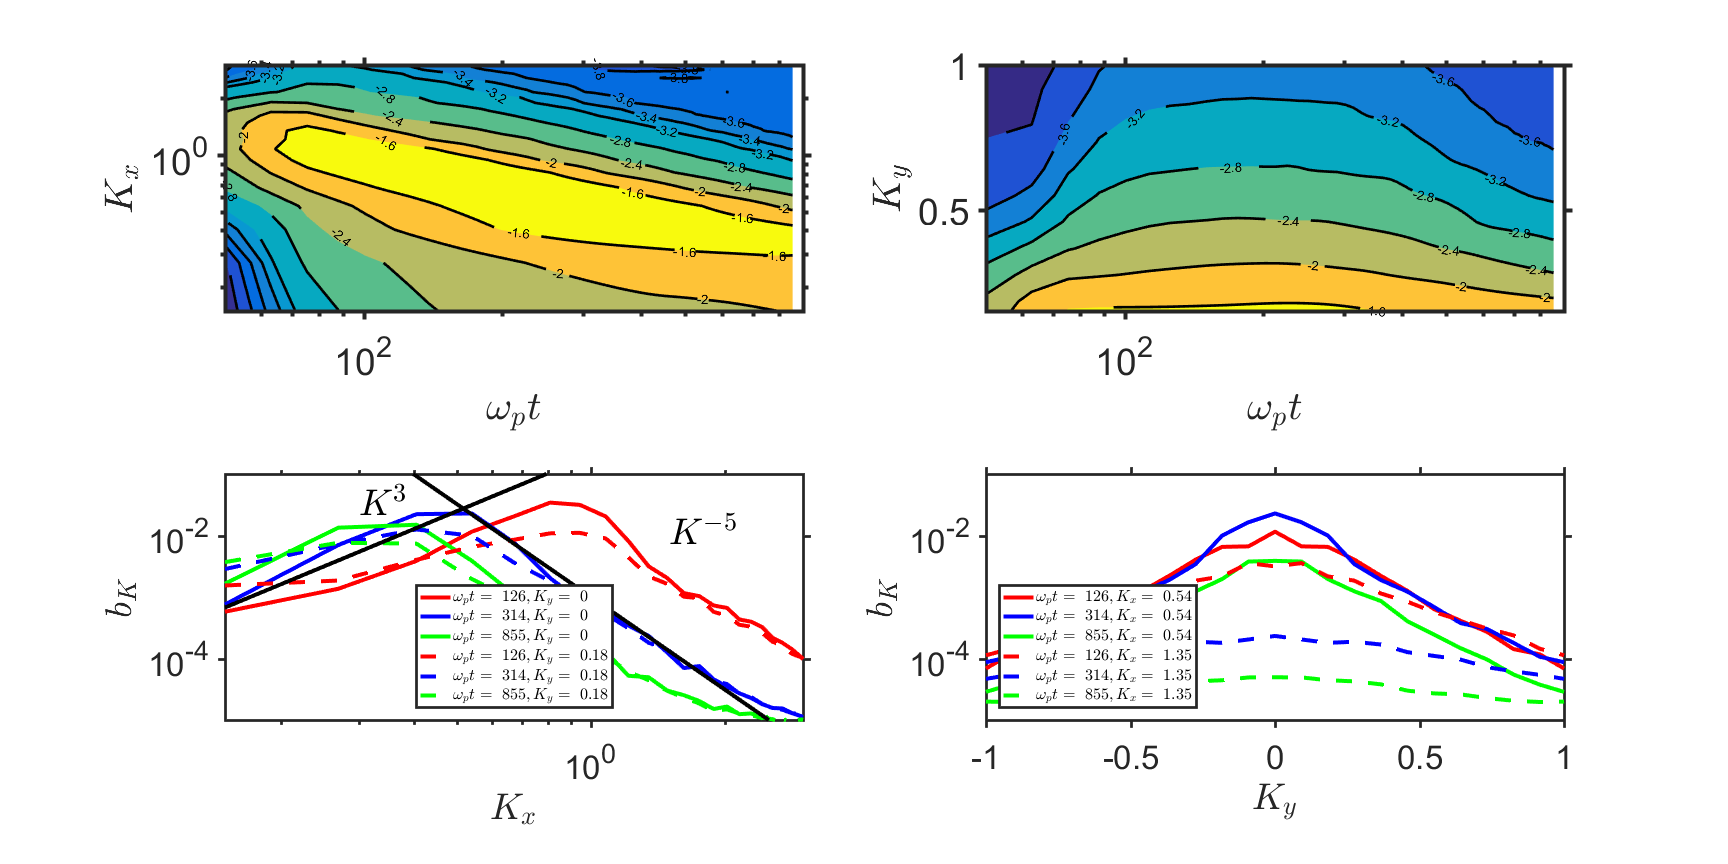
\includegraphics[width=1\linewidth]{part4/spectrA10_B0.png}
\captionstyle{normal}
\caption{Эволюция спектра турбулентности в двойном логарифмическом масштабе: (a)~линии уровня логарифма усредненных вдоль оси анизотропии амплитуд мод магнитного поля $|b_K|$; 
(b)~линии уровня логарифма усредненных поперек оси анизотропии амплитуд мод магнитного поля $|b_K|$; 
(c)~спектр $|b_K|$ магнитного поля поперек оси анизотропии при продольных волновых числах $K_\|=0$ (сплошная) и $K_\|=0.18$ (пунктир). 
(d)~спектр $|b_K|$ магнитного поля вдоль оси анизотропии при поперечных волновых числах $K_\perp=0.54$ (сплошная) и $K_\perp=1.35$ (пунктир) в моменты времени $\wpl t$, равные 126 (красный цвет), 314 (синий), 855 (зеленый). Внешнее магнитное поле отсутствует $b_{ext}=0$.
}
\label{ris:spectrA10_B0}
\end{figure}

Гармоники по-прежнему могут находиться на одной из 4 возможных стадий эволюции: экспоненциальный, степенной или сверхбысрый рост, а также осцилляционное затухание. Показатель степенного роста, который могут испытывать и нелинейно индуцированные сравнительно длинноволновые наклонные гармоники, по-прежнему оценивается от $1$ до $2$. Усреднение по аксиальному углу позволяет также выделить показатель усредненного затухания, который после добавления наклонных мод увеличивается и теперь оценивается от $-2$ до $-1.5$.  

В незамагниченной плазме продольная компонента турбулентного магнитного поля возникает исключительно вследствие нелинейной генерации. Во внешнем магнитном поле неустойчивая апериодическая мода обладает смешанной поляризацией (ни ТМ- ни ТЕ-), что существенно сближает и без того схожую и взаимосвязанную спектральную динамику поперечной и продольной компонент магнитного поля. Поэтому в последующих главах обсуждается спектр именно поперечной компоненты турбулентного магнитного поля. 


\subsection{Конкуренция вейбелевской и шланговой турбулентности и нелинейное взаимодействие мод в сравнительно слабом внешнем магнитном поле}
\label{part_spectr_b4}
Уже при $b_{ext}< b_{s\perp}$ значение линейного инкремента может оказаться существенно выше у наклонных мод апериодической неустойчивости, чем у поперечных мод, а значит, неучет наклонных мод становится невозможен. При сравнительно слабом внешнем магнитного поля $b_{ext}=0.4$~(рис. \ref{ris:spectrA10_B44}) инкремент поперечных мод все еще сравним с максимальным, но область неустойчивости как в поперечном, так и в продольном к оси анизотропии направлениях существенно уменьшается~\cite{Emelyanov2023_Radiophys,Moya2022}), а длинноволновая граница области неустойчивости становится отличной от нуля~(\ref{eq:border_perp_inst}). Помимо этого, апериодические неустойчивые моды теперь являются смешанными, то есть не являются ни ТЕ-, ни ТМ-модами. 



\begin{figure}[h]

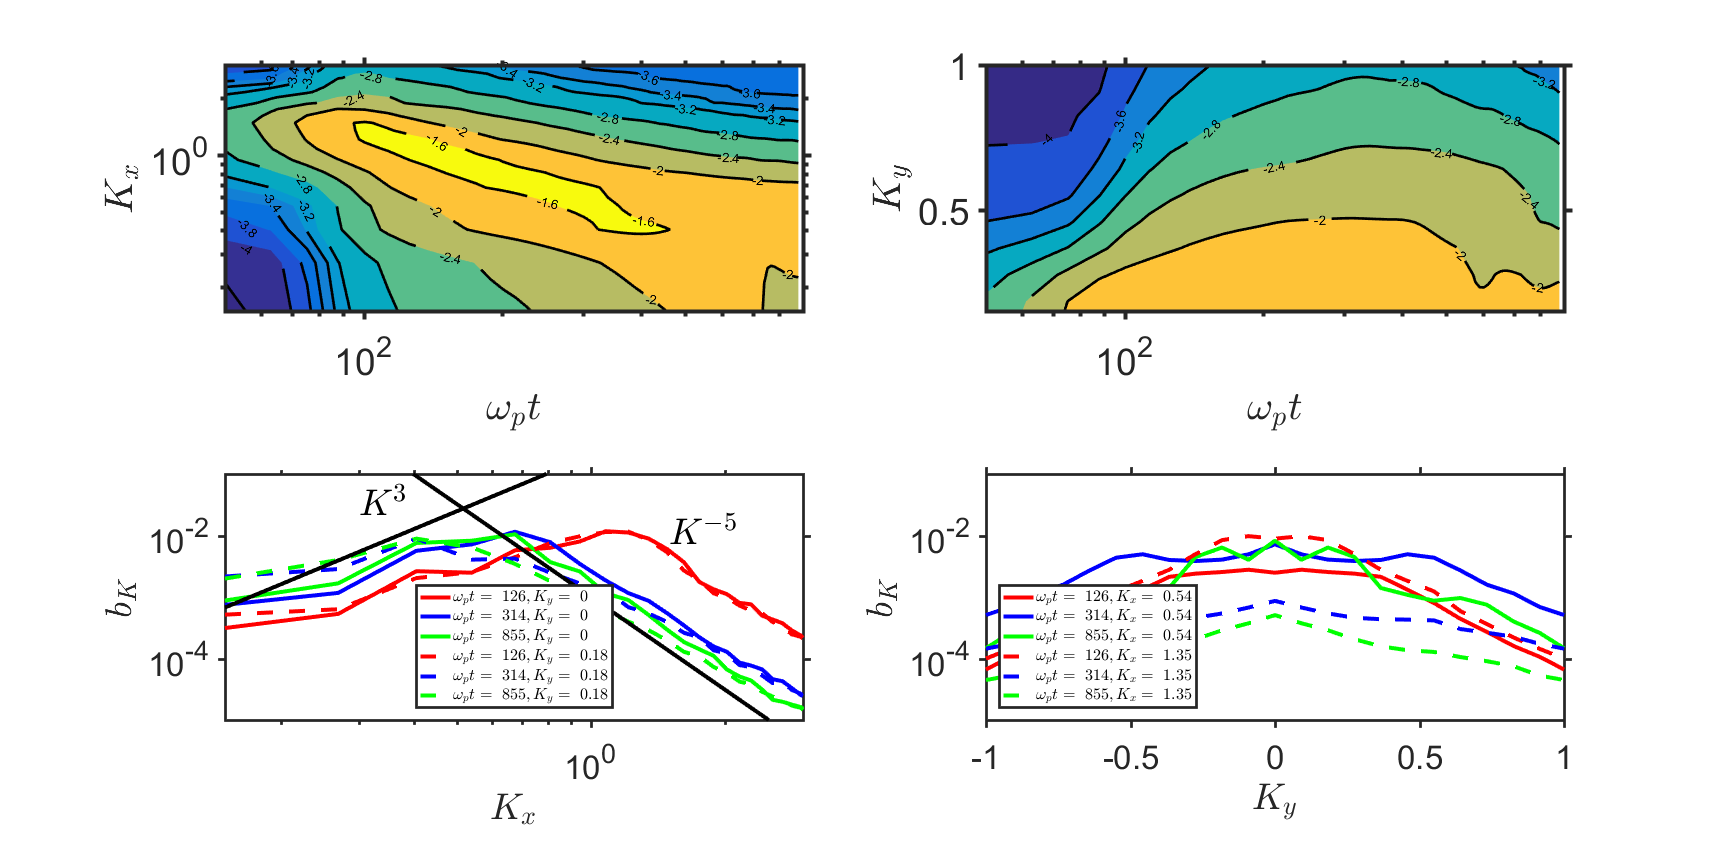
\includegraphics[width=1\linewidth]{part4/spectrA10_B44.png}
\captionstyle{normal}
\caption{Эволюция спектра турбулентности в двойном логарифмическом масштабе: (a)~линии уровня логарифма усредненных вдоль оси анизотропии амплитуд мод магнитного поля $|b_K|$; 
(b)~линии уровня логарифма усредненных поперек оси анизотропии амплитуд мод магнитного поля $|b_K|$; 
(c)~спектр $|b_K|$ магнитного поля поперек оси анизотропии при продольных волновых числах $K_\|=0$ (сплошная) и $K_\|=0.18$ (пунктир). 
(d)~спектр $|b_K|$ магнитного поля вдоль оси анизотропии при поперечных волновых числах $K_\perp=0.54$ (сплошная) и $K_\perp=1.35$ (пунктир) в моменты времени $\wpl t$, равные 126 (красный цвет), 314 (синий), 855 (зеленый). Внешнее магнитное поле $b_{ext}=0.44$.
}
\label{ris:spectrA10_B44}
\end{figure}



Из-за нелинейной генерации мод в длинноволновой области, спектр турбулентности вскоре после насыщения неустойчивости сравнительно быстро расширяется в эту область~(рис. \ref{ris:all_modes}b). Подобная сверхбыстрая генерация длинноволновых, линейно устойчивых мод, которые уже на временах, двукратно превосходящих время насыщения неустойчивости, становятся основными энергонесущими модами, отсутствует в квазилинейном приближении, что предопределяет отличную эволюцию спектра. В квазилинейных аксиально симметричных симуляциях наблюдаются лишь не затухающие колебания линейно неустойчивых мод, а смещение спектра за пределы области линейной неустойчивости отсутствует. Поэтому на временах уже двукратно превышающих момент насыщения неустойчивости спектр существенно не квазилинеен, что отражается на распределении частиц по скоростям~(ср. рис. \ref{ris:FR_A10_3d_B44} и рис. \ref{ris:FR_A10_3d_B44_QL}).



Тем не менее, многие черты квазилинейной эволюции спектральная динамика сохраняет: характерное волновое число по-прежнему смещается в длинноволновую область;  более коротковолновые моды, чем характерная в данный момент времени мода, осцилляционно затухают, а многие более длинноволновые, в том числе и нелинейно индуцированные при насыщении неустойчивости~--- нарастают по степенному закону. Затухание линейно неустойчивых гармоник замедляется в сравнении со случаем отсутствия внешнего магнитного поля и показатель их усредненного степенного затухания оценивается от $-1.3$ до $-0.8$. Показатели степенного нарастания основных энергонесущих гармоник по-прежнему лежат в промежутке от $1$ до $2$, в том числе и для некоторых нелинейно индуцированных длинноволновых мод. Исключением из обеих оценок являются длинноволновые, почти поперечные, нелинейно индуцированные моды $\left(K_x\lesssim0.6,K_y\lesssim0.1\right)$, показатели нарастания и затухания которых стремятся к нулю. Таким образом, хотя квазилинейное взаимодействие по-прежнему остается весьма существенным в присутствии внешнего магнитного поля, непосредственно вид наблюдаемого спектра турбулентного магнитного поля в значительной степени определяется прямым межмодовым нелинейным взаимодействием.


\subsection{Динамика спектра шланговой турбулентности и нелинейное взаимодействие мод в подавляющем поперечные моды внешнем магнитном поле}


Начиная с величины внешнего магнитного поля $b_{ext}=0.59$ анализ линейного дисперсионного соотношения предсказывает устойчивость поперечных мод ~(рис. \ref{ris:spectrA10_B65}). Оптимальный волновой вектор (волновой вектор с наибольшим линейным инкрементом) при $b_{ext}=0.59$ образует угол с осью анизотропии, приблизительно равный $77^\circ$, а область апериодической неустойчивости продолжает обужение как в продольном, так и в поперечном направлении. Топология области неустойчивости в трехмерном пространстве изменилась: ранее она состояла из одной связанной области, ограниченной квазитороидальной поверхностью, а теперь~--- из двух~(рис. \ref{ris:mode_coupling}). В ходе нелинейной динамики спектра, как и в работах~\cite{Camporeale2008,Hellinger2014}, наблюдается смещение его максимума в длинноволновую область и уменьшение отношения характерного поперечного волнового числа к продольному. На протяжении нелинейной эволюции существенны квазипоперечные  моды  $\left(K_\|<K_{\|opt}/2\right)$, сгенерированные в широком диапазоне волновых чисел за счет трехволнового взаимодействия линейно неустойчивых мод и нарастающие с инкрементами, близкими к удвоенному максимальному инкременту~(рис. \ref{ris:all_modes}c). К моменту насыщения неустойчивости амплитуда их магнитного поля в $2-4$ раза ниже амплитуды магнитного поля наиболее линейно неустойчивой моды, а на временах в $3-4$ раза более поздних они становятся основными энергонесущими модами. Моды с удвоенной к линейно неустойчивым модам продольной компонентой волнового вектора $\left(K_\|\approx2K_{\|opt}\right)$ генерируются за счет того же механизма в широком, сравнимом с областью линейной неустойчивости, диапазоне значений поперечной компоненты~(рис. \ref{ris:mode_coupling}b). Аналогично,  к моменту насыщения неустойчивости их амплитуда в $2-4$ раза ниже амплитуды наиболее линейно неустойчивых мод. В течение последующей эволюции часть из них может стать основными энергонесущими модами, но к концу симуляций наблюдается затухание удвоенных продольных мод. 


\begin{figure}[h!]

\includegraphics[width=1\linewidth]{part4/spectrA10_B65.png}
\captionstyle{normal}
\caption{Эволюция спектра турбулентности в двойном логарифмическом масштабе: (a)~линии уровня логарифма усредненных вдоль оси анизотропии амплитуд мод магнитного поля $|b_K|$; 
(b)~линии уровня логарифма усредненных поперек оси анизотропии амплитуд мод магнитного поля $|b_K|$; 
(c)~спектр $|b_K|$ магнитного поля поперек оси анизотропии при продольных волновых числах $K_\|=0$ (сплошная) и $K_\|=0.27$ (пунктир). 
(d)~спектр $|b_K|$ магнитного поля вдоль оси анизотропии при поперечных волновых числах $K_\perp=0.54$ (сплошная) и $K_\perp=1.35$ (пунктир) в моменты времени $\wpl t$, равные 126 (красный цвет), 314 (синий), 855 (зеленый). Внешнее безразмерное магнитное поле $b_{ext}=0.59$.
}
\label{ris:spectrA10_B65}
\end{figure}

По-прежнему выделяются 4 возможные стадии эволюции для гармоник. Линейно неустойчивые апериодические моды испытывают экспоненциальный рост в соответствии с дисперсионным соотношением. После насыщения своего роста каждая мода в отдельности осцилляционно затухает. При насыщении неустойчивости наблюдается сверхбыстрый рост поперечных и удвоенных продольных мод. 


%%В ходе дальнейшей нелинейной эволюции из-за деформации однородной компоненты функции распределения частиц по скоростям наблюдается примерно степенной рост сравнительно длинноволновых, изначально линейно устойчивых и не генерируемых нелинейно мод, с достаточно высокими показателями роста, близкими к 5. 
Область волновых чисел, в которой наблюдается степенной рост, можно грубо оценить: $K_{\|opt}\lesssim  K_\|\lesssim 2K_{\|opt}$, $0\lesssim K_\perp\lesssim 2K_{\perp opt}$. В работах~\cite{Camporeale2008,Hellinger2014} предполагается, что длинноволновое смещение спектра с уменьшением угла наклона между характерным волновым вектором и магнитным полем происходит квазилинейно, и предпринимаются попытки его объяснить на основе линейной теории. Важно, что скорость их степенного роста сравнима со скоростью экспоненциального роста линейно неустойчивых мод (а при внешнем поле $b_{ext}=0.71$ значительно превосходит), что кажется невероятным в контексте квазилинейного взаимодействия, так как наблюдаемое нарастание происходит при уже значительно изотропизованном распределении частиц по скоростям. 

%В будущем, чтобы проверить гипотезу о ключевой роли квазилинейного взаимодействия в наблюдаемом смещении основных энергонесущих мод, необходимо выяснить, неустойчиво ли среднее в пространстве распределение частиц по скоростям в обсуждаемом внешнем магнитном поле относительно мод, сравнительно быстрый степенной рост которых наблюдается при этом распределении. 

\subsection{Шланговая турбулентность и нелинейное взаимодействие мод в сильном внешнем магнитном поле}
\label{part_spectr_b78}

Оптимальный волновой вектор линейного роста апериодической неустойчивости при  $b_{ext}=0.78$ образует угол с осью анизотропии, приблизительно равный  $70^\circ$, а область неустойчивости крайне обужена около соответствующей моды. К моменту насыщения неустойчивости наблюдается нелинейная генерация не только поперечных и удвоенных продольных мод, но и гармоник с примерно утроенным и даже учетверенным оптимальным продольным волновым числом~(рис. \ref{ris:all_modes}d), что придает спектру вдоль оси анизотропии гребенчатую форму. Далее в ходе нелинейной эволюции поперечное волновое число наиболее энергонесущих мод уменьшается, а продольное~--- увеличивается. Вслед за спектральным смещением наиболее энергонесущих мод происходит пропорциональное смещение кратных индуцированных гармоник. Вследствие этого спектр сглаживается в продольном направлении, теряя гребенчатую форму. Подобный процесс происходил и при меньшем поле $b_{ext}=0.59$, но был менее заметен из-за скоротечности и более широкого спектра линейно неустойчивых мод.

\begin{figure}[h!]

\includegraphics[width=1\linewidth]{part4/spectrA10_B78.png}
\captionstyle{normal}
\caption{Эволюция спектра турбулентности в двойном логарифмическом масштабе: (a)~линии уровня логарифма усредненных вдоль оси анизотропии амплитуд мод магнитного поля $|b_K|$; 
(b)~линии уровня логарифма усредненных поперек оси анизотропии амплитуд мод магнитного поля $|b_K|$; 
(c)~спектр $|b_K|$ магнитного поля поперек оси анизотропии при продольных волновых числах $K_\|=0$ (сплошная) и $K_\|=0.37$ (пунктир). 
(d)~спектр $|b_K|$ магнитного поля вдоль оси анизотропии при поперечных волновых числах $K_\perp=0.54$ (сплошная) и $K_\perp=0.81$ (пунктир) в моменты времени $\wpl t$, равные 478 (красный цвет), 628 (синий), 855 (зеленый). Внешнее безразмерное магнитное поле $b_{ext}=0.71$.
}
\label{ris:spectrA10_B78}
\end{figure}

На протяжении линейной неустойчивости происходит экспоненциальный рост смешанных апериодических мод в соответствии с линейной теорией. При насыщении неустойчивости наблюдается нелинейная генерация квазипоперечных $\left(K_\|<K_{\|opt}/2\right)$, удвоенных $\left(K_\|\approx2K_{\|opt}\right)$ и утроенных $\left(K_\|\approx3K_{\|opt}\right)$ продольных гармоник, а также гармоник на коротковолновом хвосте области неустойчивости ($\left(K_\|\approx K_{\|opt},K_\perp\gtrsim2K_{\perp opt}\right)$). Квазипоперечные моды нарастают с инкрементами, близкими к удвоенным вследствие трехволнового взаимодействия. Подобно четырехволновой генерации утроенной моды в отсутствие внешнего магнитного поля, для нелинейной генерации гармоник на коротковолновом хвосте линейной области неустойчивости должны сложится три основные энергонесущие моды~(рис. \ref{ris:mode_coupling}b). Инкременты нелинейного роста удвоенных продольных мод оценить затруднительно из-за шумов, однако они оказывается существенно выше удвоенного линейного, что дает основание предполагать генерацию этих гармоник не только посредством простого сложения двух линейно неустойчивых мод, но и за счет нелинейных взаимодействий более высокого порядка. То же касается и генерации утроенной продольной моды (рис. \ref{ris:all_modes}d). К насыщению неустойчивости уровень квазипоперечных и удвоенных продольных мод примерно на порядок ниже основной энергонесущей моды, утроенной продольной~--- на два порядка, гармоник коротковолнового хвоста~--- примерно полтора порядка. В ходе нелинейного смещения максимума спектра в линейно устойчивую область происходит быстрая, нелинейная генерация мод, отдельные участки которой лучше аппроксимируются экспоненциальной функцией, а отдельные~--- степенной с показателем, достигающим $10$. 
\section{Условия применимости квазилинейного подхода к описанию шланговой турбулентности} 
низкое внешнее магнитное поле